\section{ТЕОРЕТИЧЕСКИЕ СВЕДЕНИЯ}

Нейронные сети представляют собой упрощенную модель головного мозга.
Мозг состоит из нейронов, которые соединяются (являясь при этом
индивидуальными процессорами) и взаимодействуют друг с другом.
В упрощенном виде работу мозга можно представить следующим образом:
из окружающей среды через сенсоры передаются импульсы (внешний слой),
средний слой обрабатывают эти импульсы. На рисунке~\ref{fig:neuron}
изображено схематичное представление нейрона.
\begin{figure}[h!]
  \centering
  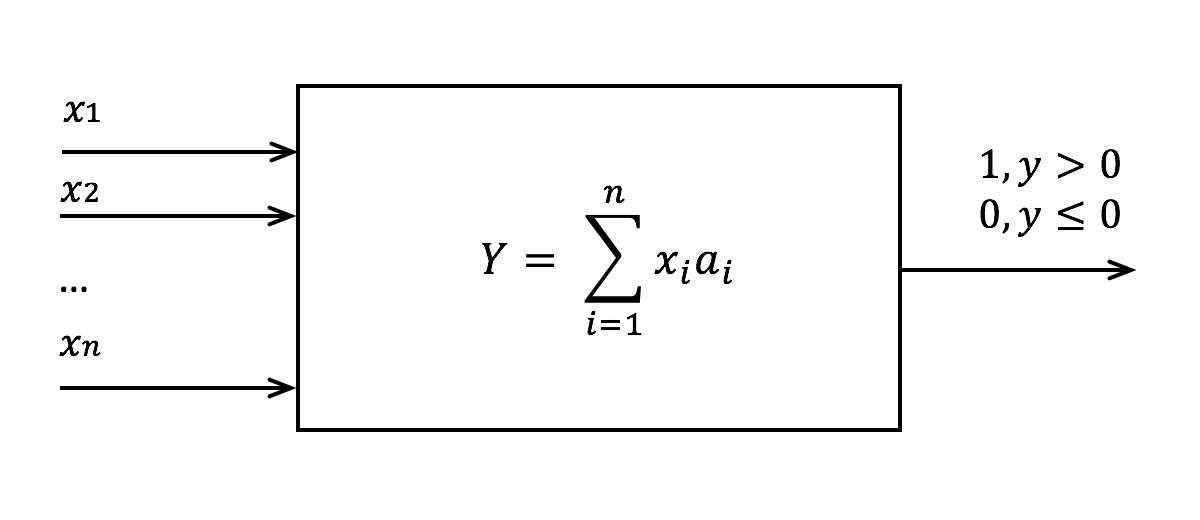
\includegraphics[width=130mm]{img/neuron}
  \caption{Схематичное представление нейрона}
  \label{fig:neuron}
\end{figure}

Коэффициенты $a_i$ определяются в ходе обучения нейрона или путём
решения системы алгебраических неравенств. Если на выходе сумма $Y$
больше нуля, то считается, что нейрон распознал входной вектор $X$,
если же сумма $Y$ меньше нуля, то входной вектор $X$ считается отклоненным.   

В 1957 году Фрэнк Розенблатт описал конструкцию, названную им персептроном.
Персептрон (англ. perceptron --- восприятие) --- математическая
или компьютерная модель восприятия информации мозгом (кибернетическая
модель мозга), реализованная в виде электронной машины <<Марк-1>> в 1960 году.

По Розенблатту персептрон состоит из трех слоев нейронов.
Первый слой --- это сенсорные элементы, которые задают, что же мы имеем на входе.
Второй слой –-- ассоциативные элементы. Их связи с сенсорным слоем жестко
заданы и определяют переход к более общей, чем на сенсорном слое,
ассоциативной картине описания.

Обучение персептрона осуществляется за счет изменения весов нейронов
третьего реагирующего слоя. Цель обучения --– заставить персептрон
правильно классифицировать подаваемые образы.
Нейроны третьего слоя работают как пороговые сумматоры.
Соответственно, веса каждого из них определяют параметры некой гиперплоскости.
Если есть линейно-разделимые входные сигналы, то выходные нейроны
как раз и могут выступать как их классификаторы.

Формула реализуемой персептроном дискриминаторной функции имеет вид:
\begin{equation}
\label{eq:Y}
  Y = a_0 + a_1 \: x_1 + a_2 \: x_2 + \dots + a_n \: x_n,
\end{equation}
где \hspace{2mm} $a_i$ --- весовые коэффициенты при переменных, \par
$x_i$ --- сигналы с датчиков.

\newpage